%%%%%%weekly meeting template, prepared by Isaac Lee.  02/08/2017
\documentclass[11pt, a4paper]{article}
\usepackage{times}
\usepackage{ifthen}
\usepackage{amsmath}
\usepackage{amssymb}
\usepackage{graphicx}
\usepackage{setspace}

%%% page parameters
\oddsidemargin -0.5 cm
\evensidemargin -0.5 cm

\renewcommand{\baselinestretch}{0.4}\normalsize
\setlength{\parskip}{0pt}

\begin{document}
%%%mention the no, time, and venue of the meeting
\noindent Software Engineering Group Project PG 29 {\bf Client Meeting} on {\bf Tuesday 08/08/2017}.
\vspace*{10pt}
\begin{center}
\huge \bf Agenda
\end{center}

%%%first, nominate a chair for the meeting. We suggest that each member at least has one chance as the chair.
\section{Attendees}
\begin{itemize}
\item Chair: Ben
\item Facilitator: Pavi
\item TimeKeeper: Sean
\item Recorder: Isaac
\item Sammy
\item Huy Nguyen
\end{itemize}
%%%if some students cannot make the meeting due to some reasons, their names should appear here.

\section{Client Questions}
\subsection{The Rover Map}
\begin{itemize}
	\item What does the map look like, physical obstacles and lines?
	\item Is the starting location and orientation of the robot known?
	\item How much of the map do we explore?
	\item How is accuracy measured?
	\item When this DTD for the xml completed? Is there any ETA?
	\item Details on the starting point for partially completed maps
\end{itemize}

\subsection{No Go Zones}
\begin{itemize}
	\item How are the No Go Zones intended to be selected on the UI?
	\item Are they represented physically or just graphically on the map?
	\item What is used by the operator to display the map and control the robot?
	\item What are the consequences of moving out side the map? or NGZ or craters?
\end{itemize}

\subsection{Simulated Terrain}
\begin{itemize}
	\item How wide are the lines on the map?
	\item What colours/shapes indicate craters, trails?
	\item What is definition of mission accomplished?
	\item Do tracks/trails exist inside survey area or border only?
	\item What is the landing size?
\end{itemize}

\subsection{Operation of Rover}
\begin{itemize}
	\item Details on robot interfaces and sensors?
	\item How does the operator give commands to robot?
\end{itemize}

\subsection{Safety}
\begin{itemize}
	\item What indicates an external object?
	\item What is the definition of a "collision" and "significant" force?
\end{itemize}

\section{Initial System Overview}
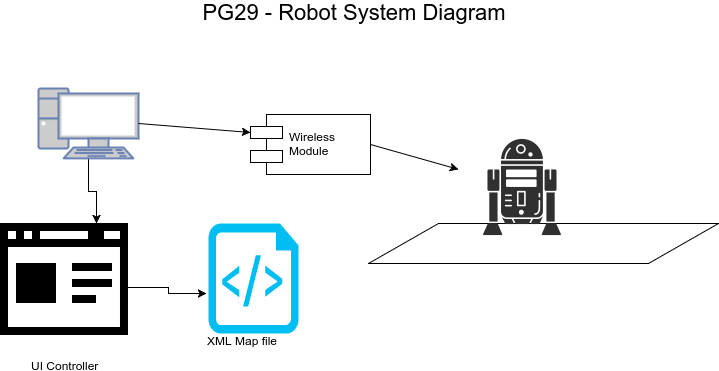
\includegraphics[width=\textwidth]{system-flowchart}

\section{Negotiation}
\begin{itemize}
	\item What milestones are most important?
\end{itemize}

\section{Next meeting}

\section {Close meeting}
%%%finally, specifies time of next meeting
\vspace*{10pt}


\end{document}
